\documentclass[12pt]{article}

\usepackage[spanish]{babel}
\usepackage[utf8]{inputenc}
\usepackage[right=1.5cm,left=1.5cm,top=1.5cm,bottom=1.5cm]{geometry}

\title{Tercer Taller\\ Estadística genómica}
\author{Juan David Henao Sánchez}

\usepackage{Sweave}
\begin{document}
\Sconcordance{concordance:JuanHenao_Taller3.tex:JuanHenao_Taller3.Rnw:%
1 9 1 1 0 9 1 1 2 1 0 1 1 3 0 2 2 1 0 2 1 7 0 1 1 19 0 1 1 7 0 2 2 4 0 %
2 2 1 0 1 1 4 0 2 2 1 0 1 1 4 0 1 2 5 1 1 2 1 0 4 1 5 0 1 1 6 0 2 2 1 0 %
2 1 4 0 1 2 5 1 1 2 4 0 2 2 1 0 1 1 6 0 2 2 4 0 2 2 1 0 2 1 1 2 4 0 1 2 %
1 1}


\maketitle

\section*{Sobre datos del GEO del NCBI de su elección (que comparen dos condiciones biológicas con al menos 5 réplicas) realice los siguientes pasos luego de normalizar:}
\subsection*{1. Realice un MA-plot}

\begin{itemize}
\item{Carga de librerias}
\begin{Schunk}
\begin{Sinput}
> library(GEOquery)
> library(vsn)
\end{Sinput}
\end{Schunk}
\item{Extrayendo datos}
\begin{Schunk}
\begin{Sinput}
> gds <- getGEO("GDS3750")
> eset <- GDS2eSet(gds, do.log2 = TRUE)
> class(eset)
\end{Sinput}
\begin{Soutput}
[1] "ExpressionSet"
attr(,"package")
[1] "Biobase"
\end{Soutput}
\begin{Sinput}
> eset
\end{Sinput}
\begin{Soutput}
ExpressionSet (storageMode: lockedEnvironment)
assayData: 22277 features, 8 samples 
  element names: exprs 
protocolData: none
phenoData
  sampleNames: GSM430339 GSM430340 ... GSM430346 (8 total)
  varLabels: sample genotype/variation description
  varMetadata: labelDescription
featureData
  featureNames: 1007_s_at 1053_at ... AFFX-TrpnX-M_at (22277 total)
  fvarLabels: ID Gene title ... GO:Component ID (21 total)
  fvarMetadata: Column labelDescription
experimentData: use 'experimentData(object)'
  pubMedIds: 20395301 
Annotation:  
\end{Soutput}
\begin{Sinput}
> dim(eset)
\end{Sinput}
\begin{Soutput}
Features  Samples 
   22277        8 
\end{Soutput}
\end{Schunk}
\item{Normalización}
\begin{Schunk}
\begin{Sinput}
> nml <- justvsn(eset)
\end{Sinput}
\end{Schunk}
\item{Grafica de datos No normalizados}
\begin{Schunk}
\begin{Sinput}
> meanSdPlot(eset)
> title(main='Datos No normalizados',font=2)
\end{Sinput}
\end{Schunk}
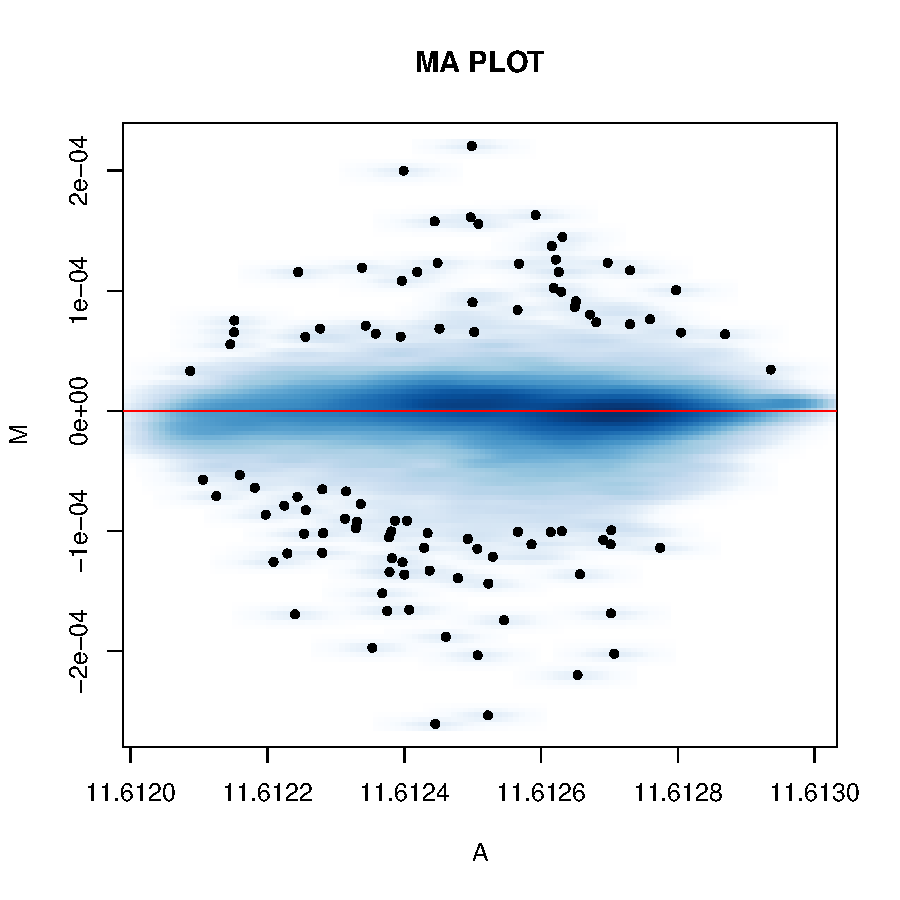
\includegraphics{JuanHenao_Taller3-004}
\item{Grafica de datos normalizados}
\begin{Schunk}
\begin{Sinput}
> meanSdPlot(nml)
> title(main='Datos normalizados',font=2)
\end{Sinput}
\end{Schunk}
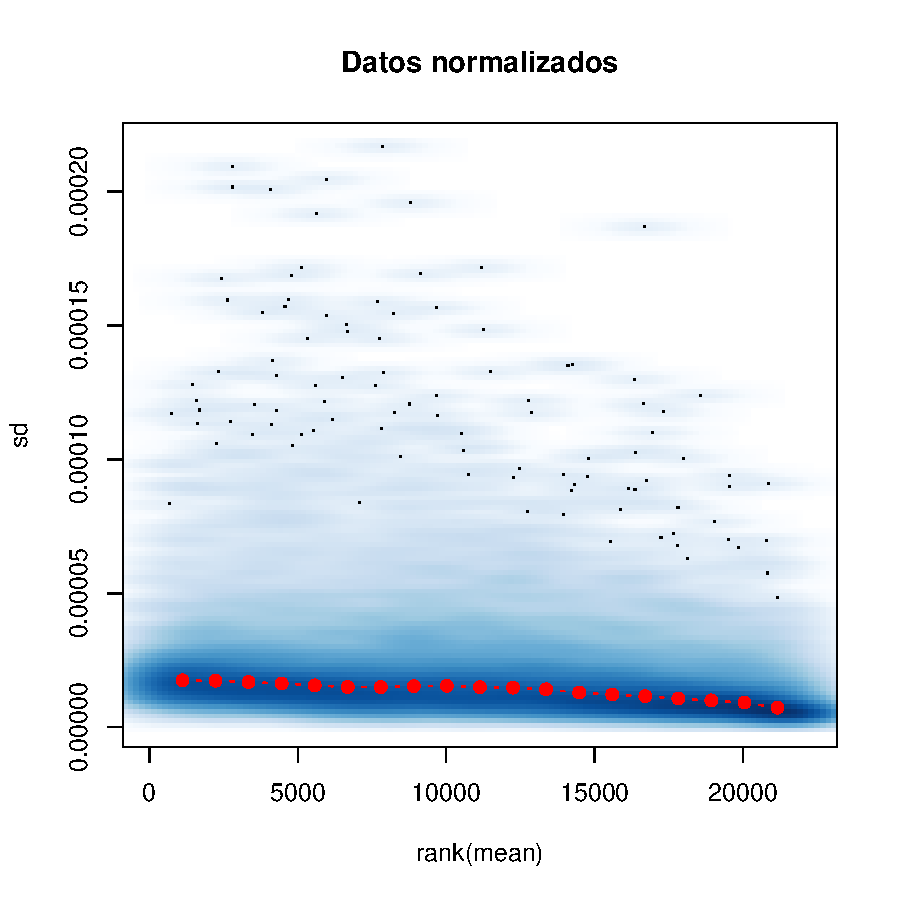
\includegraphics{JuanHenao_Taller3-005}
\end{itemize}

\textbf{MA PLOT}

\begin{itemize}
\item{Calculando variables}
\begin{Schunk}
\begin{Sinput}
> iref = seq(1, 7, by=2)
> ismp = seq(2, 8, by=2)
> M= exprs(nml)[,ismp]-exprs(nml)[,iref]
> A=(exprs(nml)[,ismp]+exprs(nml)[,iref])/2
> dim(M)
\end{Sinput}
\begin{Soutput}
[1] 22277     4
\end{Soutput}
\begin{Sinput}
> dim(A)
\end{Sinput}
\begin{Soutput}
[1] 22277     4
\end{Soutput}
\end{Schunk}
\item{Generando la grafica}
\begin{Schunk}
\begin{Sinput}
> smoothScatter(rowMeans(A), rowMeans(M), main=" ", xlab="A", ylab="M")
> title(main='MA PLOT',font=2)
> abline(h=0, col="red")
\end{Sinput}
\end{Schunk}
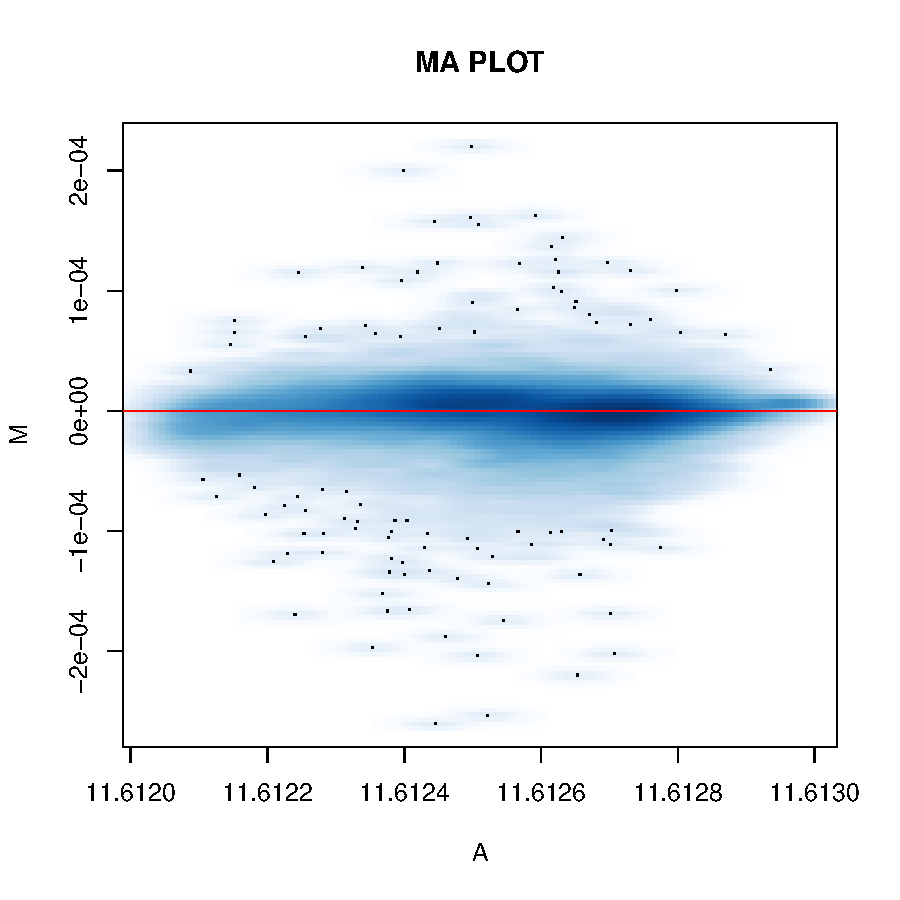
\includegraphics{JuanHenao_Taller3-007}
\end{itemize}

\subsection*{2. Identifique los genes diferencialmente expresados con pruebas T múltiples (rowttest) y resáltelos en el MAplot}

\begin{itemize}
\item{Cargando la libreria necesaria}
\begin{Schunk}
\begin{Sinput}
> library(genefilter)
\end{Sinput}
\end{Schunk}
\item{Eliminando los datos N/A}
\begin{Schunk}
\begin{Sinput}
> Expresados <- exprs(nml)[complete.cases(exprs(nml)),]
> dim(Expresados)
\end{Sinput}
\begin{Soutput}
[1] 22277     8
\end{Soutput}
\end{Schunk}
\item{Aplicando la prueba T múltiple}
\begin{Schunk}
\begin{Sinput}
> PruebaT<-rowttests(Expresados[,c(1:8)],factor(c(0,0,0,0,1,1,1,1)))$p.value<0.05
\end{Sinput}
\end{Schunk}
\item{Resaltándo los genes diferencialmente expresados}
\begin{Schunk}
\begin{Sinput}
> smoothScatter(rowMeans(A), rowMeans(M), main=" ", xlab="A", ylab="M")
> title(main='MA PLOT',font=2)
> abline(h=0, col="red")
> points(rowMeans(A[PruebaT,]),rowMeans(M[PruebaT,]),col="red",cex=0.1)
\end{Sinput}
\end{Schunk}
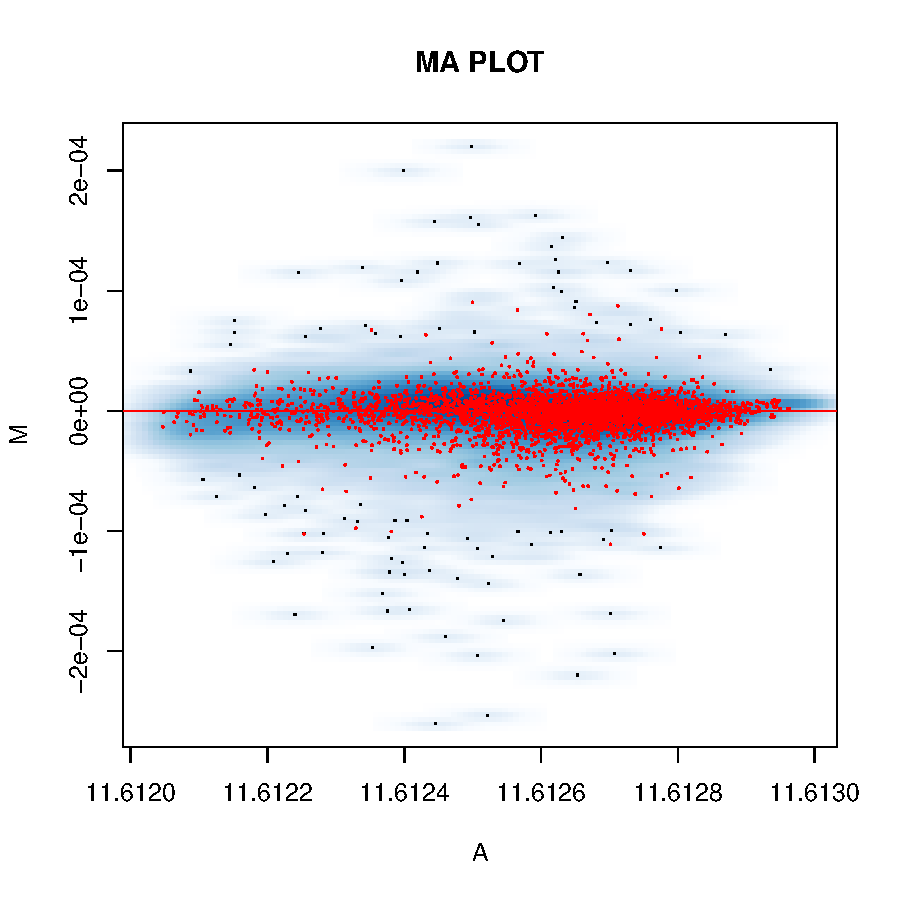
\includegraphics{JuanHenao_Taller3-011}
\end{itemize}
\end{document}
